\documentclass{article}

\usepackage{multicol}
\usepackage{graphicx}
\usepackage{caption}
\usepackage{hyperref}

\usepackage[left=2cm,right=2cm,top=2cm,bottom=2.5cm]{geometry}

\title{\textbf{MATH 300 Final Project}}
\author{Ali Hamza $|$ Maham Shoaib $|$ Hassan Naseem}
\date{\today}

\begin{document}
\maketitle

\section{Tasks}
\subsection{Task 1}
In this section we made a function $task1(steps,start,leftprob,stopprob)$. The function takes steps using an algorithm that makes use
of an algorithm that can be explained using the following diagram.
\begin{center}
    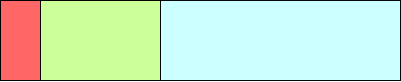
\includegraphics{task1prob.png}
\end{center}
Let us assume
\begin{itemize}
    \item The red region is the probability of not moving
    \item The green region is the probability of moving left
    \item The blue region is the probability of moving right
\end{itemize}
The algorithm simply checks if the randomly generated numbers $0\leq n \leq 1$ lies within a certain 
region and makes movement accordingly.\\\\
Running the algorithm on multiple steps the following graphs were obtained.
To find the expected average distance at a certain step the we ran multiple simulations of the code and calculated an average step at each step. This rendered
the following random walk that is made up of average steps. This is then an expected
random walk. 
%include graph here

\subsection{Task 2}
In task 2 we took a similar approach as task 1. The only difference was that we simulated a random walk 
for two particles on the same graph. However, the same issues of randomness arose and it was impossible to
predict the average step at which the two particles met. 
\\\\
Similar, to task 1 we simulated multiple random walks of the two particles and calculated the average step 
at which the particles were meeting for a certain number of steps and distance. The data of each intercepting 
step was recorded into an array and the average was calculated to find an expected intercepting step.
\\\\
We also plotted the average random walks of the the two particles and the result of that was as follows:
It is worth noting, however, that this graph is also subject to change based on different parameters. However, 
it seems to be stable on multiple executions. There is some deviation though. 
%Include graph here
\subsection{Task 3}
In order to determine the step size and the orientation, we assumed that the step size is a discreet random variable between {0, 0.5, 1} and orientation is a discreet random variable between {0, $\frac{\pi}{2}$, $\pi$, $\frac{3\pi}{2}$, $2\pi$}. We have used directional words such as right referring to orientation of 0 as well as $2\pi$ and up referring to $\frac{\pi}{2}$, etc. 
\\\\
We have used an algorithm similar to those used in the previous tasks to determine the probability of a step size and orientation being used. In the case of the particle exceeding the 100 $unit^{2}$ region, the particle just reverses the direction that it was moving and bounces back into the region. The trajectory is then plotted on a 3 dimensional plane.
\subsection{Task 4}
For this section we have repeated a similar procedure to that used in Task 1 except that in this case the step size is a continuous random variable between 0-1 determined by the built-in \textbf{randi} function that chooses a a number within the range with a uniform probability distribution.
\subsection{Task 5}
This section is done in a similar manner to that of Task 3, however in this case both the step size and orientation are continuous random variables between 0-1 and 0-2$\pi$ respectively. The variables were chosen in a similar manner to those in Task 4 by employing the \textbf{randi} function.
\subsection{Task 7}
In this task we have used a similar algorithm to that in Task 3 with the only exception that the orientation is a continuous random variable between 0-2$\pi$ which is chosen in a similar manner to that in Task 4 by employing the \textbf{randi} function. 
\subsection{Task 8}
\section{Bibliography}

\begin{enumerate}
    \item \url{https://www.mathworks.com/help/matlab/math/multidimensional-arrays.html}
\end{enumerate}

\section{Extras}
\begin{enumerate}
    \item Simulation video of random walk in 2D: \url{https://youtu.be/99tQ8SE9IXw}
\end{enumerate}

\end{document}
